\documentclass{beamer}
\usepackage{HECbeamer}
% \usepackage{pgfpages}
% \pgfpagesuselayout{4 on 1}[letterpaper, landscape, border shrink=5mm]
\title[\color{white}{MATH 60604A \S~6e - Random slope model}]{\texorpdfstring{MATH 60604A \\Statistical modelling \\ \S~6e - Random slope model}{MATH 60604A \\Statistical modelling \\ \S~6e - Random slope model}}
\author{Léo Belzile}
\institute{HEC Montréal\\
Department of Decision Sciences}
\date{} 

\begin{document}
\frame{\titlepage}
\begin{frame}
\frametitle{Model formulation}
 We consider a linear mixed model with a random slope and a random intercept for the \code{revenge} data, of the form 
  \begin{align*}
  \bs{Y}_i \mid \bs{\mathcal{B}}_i =\bs{b}_i &\sim \mathsf{No}_{5}\left( \mathbf{X}_i \bs{\beta} + \mathbf{Z}_i\bs{b}_i, \sigma^2 \mathbf{I}_5\right) \\
  \bs{\mathcal{B}}_i & \sim \mathsf{No}_{2}( \bs{0}_2, \bs{\Omega})
 \end{align*}
where $\mathbf{Z}_i = [\bs{1}_5, \code{time}_i]$ is a $5 \times 2$ model matrix for the random effects and $\bs{\Omega} = \big( \begin{smallmatrix}\omega_{11} & \omega_{12} \\ \omega_{12} & \omega_{22}\end{smallmatrix}\big)$.

The columns of $\mathbf{Z}_i$ typically include  as covariates
\bi \item time or 
\item indicators for categorical variables (group effect).
\ei
\end{frame}
\begin{frame}
\frametitle{Random effects on the predictor variables}
Suppose the matrix $\mathbf{Z}_i = [\bs{1}_{n_i}, \mathbf{X}_{1i}]$. 
\begin{align*}
Y_{ij}=(\beta_0 +\alert{b_{0i}}) + (\beta_1+\alert{b_{1i}})\mathrm{X}_{ij1}+\beta_2\mathrm{X}_{ij2}+\cdots+\beta_p\mathrm{X}_{ijp} + \varepsilon_{ij}.
\end{align*}
\bi
\item The conditional effect of the variable $\mathrm{X}_1$ \alert{for group $i$} is $\beta_1 + b_{1i}$
\item The parameter $\beta_1$ is the ``slope'' of $\mathrm{X}_1$ averaged over the entire population.
\item $\beta_1+b_{1i}$ is the effect of $\mathrm{X}_1$ specific to group $i$.
\ei
\end{frame}
\begin{frame}
\frametitle{Covariance of the response}
\bi
\item The covariance matrix of $Y_{ij}$ depends on the predictors in $\mathbf{Z}_i$ which have random effects.
\item For example, if $\mathbf{Z}_{i} = [\bs{1}_{n_i}, \mathbf{X}_{1i}]$, the marginal variance of $Y_{ij}$ is
\begin{align*}
\Va{Y_{ij}\mid \mathbf{X}_i}=\omega_{11}+\mathrm{X}_{ij1}^2 \omega_{22} + 2\mathrm{X}_{ij1} \omega_{12}+\sigma^2_{\varepsilon}.
\end{align*}
\item With independent errors, the covariance between two observations in the same group is
\begin{align*}
\Co{Y_{ij}, Y_{ik}\mid \mathbf{X}_i}=\omega_{11}+\mathrm{X}_{ij1}\mathrm{X}_{1ik}\omega_{22}+(\mathrm{X}_{ij1}+\mathrm{X}_{1ik})\omega_{12}.
\end{align*}
\item It may be difficult to estimate parameters if the errors has a complex covariance structure (not to mention computational costs).
\ei
\end{frame}

\begin{frame}[fragile]
\begin{tcolorbox}[colback=white, colframe=hecblue, title=\SASlang{} code for random slope model]
\begin{verbatim}
proc mixed data=statmod.revenge;
class id;
model revenge = sex age vc wom t / solution;
random intercept t / subject=id type=un v=1 vcorr=1;
run;
\end{verbatim}
\end{tcolorbox}
The output includes information about the number of covariance parameters, the number of random effects, etc.
\begin{center}
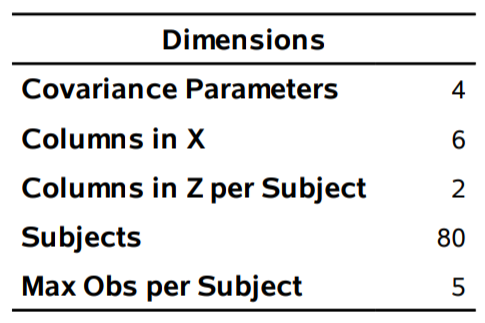
\includegraphics[width = 0.35\linewidth]{img/c6/slides7-e23}
\end{center}
\end{frame}
% \begin{frame}
%  
% \end{frame}


\begin{frame}
 \frametitle{Covariance matrix of response}
 \begin{center}
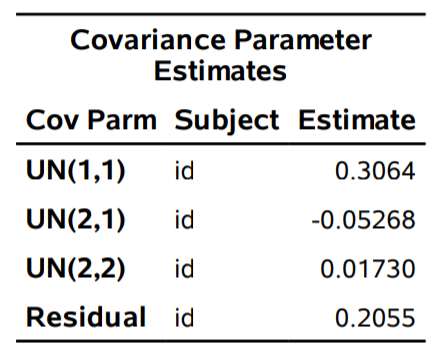
\includegraphics[width = 0.4\linewidth]{img/c6/slides7-e25}
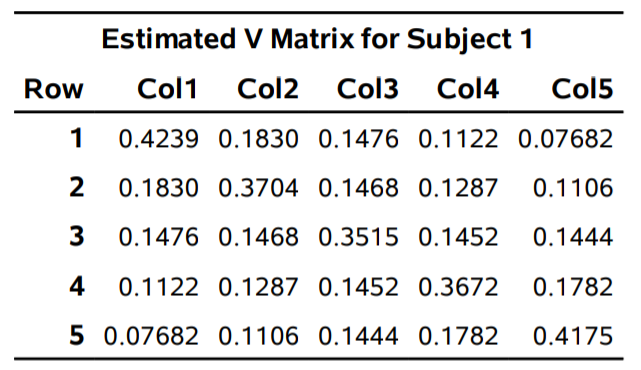
\includegraphics[width = 0.55\linewidth]{img/c6/slides7-e24}
\end{center}
\bi \item 
The variance of the random intercept is $\omega_{11}=0.3064$
\item The variance of the random slope is $\omega_{22}=0.01730$
\item The correlation between the random effects is $-0.72$.
\ei
\end{frame}
\begin{frame}
\frametitle{Testing for correlation between random effects}
\bi
\item We can test whether $\Hy_0: \omega_{12}=0$ versus $\Hy_a: \omega_{12} \neq 0$ by fitting the model with diagonal covariance and performing a likelihood ratio test (REML, since they have the same fixed effects) 
\bi
\item in \SASlang{}, change \code{type=un} to \code{type=vc} (default option)
\item the test statistic is $R=8.98$ 
\item its null distribution is $\chi^2_1$ (regular problem, covariance can be negative)
\item the $p$-value is $0.002$:
\item the correlation between the random effects is strongly significant. \ei
\ei
\end{frame}
\begin{frame}
\frametitle{Model comparison}
\bi \item 
 We can do similar comparisons with the random intercept-only model,
 \bi \item this corresponds to $\Hy_0: \omega_{22}=0$, so $\frac{1}{2}\chi^2_1$ for uncorrelated random errors.
 \item for correlated errors, setting one of the two variance parameters to zero forces $\omega_{12}=0$ and one additional parameter is lost\ldots
 \item the asymptotic null distribution approximation is complicated, 
 \begin{quote} Andrews, D.W. (2001), \textsl{Testing when a parameter is on the boundary of the maintained hypothesis}, Econometrica, 69 (3)
  \end{quote}
The approximation is also poor \ldots most people thus resort to the use of information criteria.
 \ei
 \ei
\end{frame}


\end{document}
